%%%%%%%%%%%%%%%%%%%%%%%%%%%%%%%%%%%%%%%%%
% Short Sectioned Assignment
% LaTeX Template
% Version 1.0 (5/5/12)
%
% This template has been downloaded from:
% http://www.LaTeXTemplates.com
%
% Original author:
% Frits Wenneker (http://www.howtotex.com)
% Modified by
% Peiyong Wang
% License:
% CC BY-NC-SA 3.0 (http://creativecommons.org/licenses/by-nc-sa/3.0/)
%
%%%%%%%%%%%%%%%%%%%%%%%%%%%%%%%%%%%%%%%%%

%----------------------------------------------------------------------------------------
%	PACKAGES AND OTHER DOCUMENT CONFIGURATIONS
%----------------------------------------------------------------------------------------

\documentclass[paper=a4, fontsize=11pt]{scrartcl} % A4 paper and 11pt font size
    \usepackage{amsmath,amsfonts,graphicx}
    %\usepackage{fancyhdr}
    \usepackage{booktabs}
    %\usepackage{fancyhdr}	% Required for custom headers
    \usepackage{lastpage}	% Required to determine the last page for the footer
    \usepackage{extramarks} % Required for headers and footers

    %\usepackage{algpseudocode}
    \usepackage{algorithm}
    \usepackage{algorithmicx}
    \usepackage{algpseudocode}
    \usepackage[top=2.6cm, bottom=2.6cm, left=2cm, right=2cm]{geometry}
    
    \usepackage{listings}
    \usepackage{color}
    \usepackage{xcolor}
    \definecolor{dkgreen}{rgb}{0,0.6,0}
    \definecolor{gray}{rgb}{0.5,0.5,0.5}
    \definecolor{mauve}{rgb}{0.58,0,0.82}
    \lstset{frame=tb,
         %language=Java,
         aboveskip=3mm,
         belowskip=3mm,
         showstringspaces=false,
         columns=flexible,
         basicstyle = \ttfamily\small,
         numbers=none,
         numberstyle=\tiny\color{gray},
         keywordstyle=\color{blue},
         commentstyle=\color{dkgreen},
         stringstyle=\color{mauve},
         breaklines=true,
         breakatwhitespace=true,
         tabsize=3
    }
    
    %\usepackage[]{algorithm2e}
    
    \usepackage[T1]{fontenc} % Use 8-bit encoding that has 256 glyphs
    \usepackage{fourier} % Use the Adobe Utopia font for the document - comment this line to return to the LaTeX default
    \usepackage[english]{babel} % English language/hyphenation
    \usepackage{amsmath,amsfonts,amsthm} % Math packages
    
    \usepackage{lipsum} % Used for inserting dummy 'Lorem ipsum' text into the template
    
    \usepackage{sectsty} % Allows customizing section commands
    \allsectionsfont{\centering \normalfont\scshape} % Make all sections centered, the default font and small caps
    
    \usepackage{fancyhdr} % Custom headers and footers
    \pagestyle{fancyplain} % Makes all pages in the document conform to the custom headers and footers
    \fancyhead[L]{\textsc{INFO90002 Assignment 2}}
    \fancyhead[R]{\textsc{Student Number: 955986}} % No page header - if you want one, create it in the same way as the footers below
    \fancyfoot[L]{} % Empty left footer
    \fancyfoot[C]{} % Empty center footer
    \fancyfoot[R]{\textsc{Page} \thepage \textsc{ of} \pageref{LastPage}} % Page numbering for right footer
    \renewcommand{\headrulewidth}{0pt} % Remove header underlines
    \renewcommand{\footrulewidth}{0pt} % Remove footer underlines
    \setlength{\headheight}{13.6pt} % Customize the height of the header
    
    \numberwithin{equation}{section} % Number equations within sections (i.e. 1.1, 1.2, 2.1, 2.2 instead of 1, 2, 3, 4)
    \numberwithin{figure}{section} % Number figures within sections (i.e. 1.1, 1.2, 2.1, 2.2 instead of 1, 2, 3, 4)
    \numberwithin{table}{section} % Number tables within sections (i.e. 1.1, 1.2, 2.1, 2.2 instead of 1, 2, 3, 4)
    
    \setlength\parindent{0pt} % Removes all indentation from paragraphs - comment this line for an assignment with lots of text
    % Set up the header and footer
    %\pagestyle{fancy}
   % \lhead{\textsc{INFO90002}} % Header Left
    %\chead{\textsc{The University of Melbourne}} % Header Center
    %\rhead{S\textsc{tudentNumber}: 955986} % Header Right
    %\lfoot{} % Footer Left
    %\cfoot{} % Footer Center
    %\rfoot{} % Footer Right
    %----------------------------------------------------------------------------------------
    %	TITLE SECTION
    %----------------------------------------------------------------------------------------
    
    \newcommand{\horrule}[1]{\rule{\linewidth}{#1}} % Create horizontal rule command with 1 argument of height
    
    \title{	
    \normalfont \normalsize 
    \textsc{The University of Melbourne } \\ [25pt] % Your university, school and/or department name(s)
    \horrule{0.5pt} \\[0.05cm] % Thin top horizontal rule
    \huge INFO90002 Database Systems and Information Modelling SM2, 2018
    Assignment 2 \\ % The assignment title
    \horrule{1pt} \\[0.1cm] % Thick bottom horizontal rule
    }
    
    \author{Peiyong Wang $\,$ 955986} % Your name
    
    \date{\normalsize\today} % Today's date or a custom date
    
    \begin{document}
 

    %\pagestyle{plain}
    \maketitle % Print the title
    \thispagestyle{empty}
    
    \section{ }
    \paragraph{Q1}What is the longest student name? (The length of a student’s name is the sum of the lengths of their given and family names)
    \begin{center}
        \begin{minipage}{10cm}
        \begin{tabbing}
            \hspace*{.25in} \= \hspace*{.25in} \= \hspace*{.25in} \= \hspace*{.25in} \= \hspace*{.25in} \=\kill
            {\color{blue}SELECT `givenName`, `familyName` FROM `Student`}\\
            \> {\color{blue}ORDER BY LENGTH(`givenName`) + LENGTH(`familyName`)} \\
            \> {\color{blue}DESC LIMIT 1};
        
        \end{tabbing}
        \end{minipage}
    \end{center}
    
    \begin{figure}[htbp!]
    		\centering
    		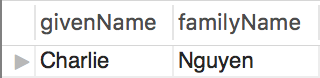
\includegraphics[width=0.6\textwidth]{q11.png}
    		\caption{Results for question one}%\label{1}
    		\vspace{-1em}
    \end{figure}

    {\color{red} One row returned}.

    \section{}
    \paragraph{Q2}List the names of students who have not yet entered any free times.
    \begin{center}
        \begin{minipage}{10cm}
        \begin{tabbing}
            \hspace*{.25in} \= \hspace*{.25in} \= \hspace*{.25in} \= \hspace*{.25in} \= \hspace*{.25in} \=\kill
            {\color{blue}SELECT `givenName`, `familyName` FROM `Student`}\\
            \> {\color{blue}LEFT JOIN `Availability` ON `Student`.`id` = `Availability`.`Student`} \\
            \> {\color{blue}WHERE `Availability`.`Student` IS NULL;}
        
        \end{tabbing}
        \end{minipage}
    \end{center}
    \begin{figure}[htbp!]
        \centering
        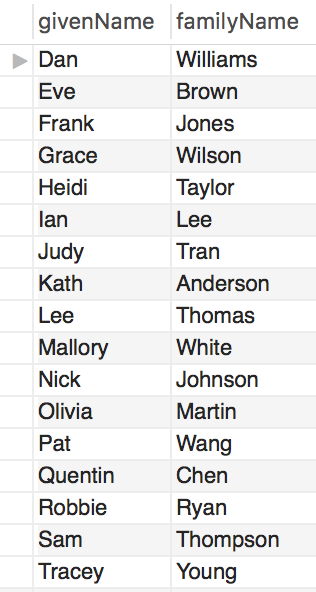
\includegraphics[width=0.5\textwidth]{q22.png}
        \caption{Results for question two}%\label{1}
        \vspace{-1em}
    \end{figure}
    \newpage
    {\color{red} 17 rows returned.}
    %\newpage
    \section{ }
    \paragraph{Q3}Which students are free on Wednesday at 10am? (show id and name)
    \begin{center}
        \begin{minipage}{10cm}
        \begin{tabbing}
            \hspace*{.25in} \= \hspace*{.25in} \= \hspace*{.25in} \= \hspace*{.25in} \= \hspace*{.25in} \=\kill
            {\color{blue}SELECT `Student`.* FROM `Student`, `Availability`}\\
            \> {\color{blue}WHERE `Student`.`id` = `Availability`.`Student`} \\
            \> {\color{blue}AND `Availability`.`hour` = 10}\\
            \> {\color{blue} AND `Availability`.`day` = 'Wed';}
        
        \end{tabbing}
        \end{minipage}
    \end{center}
    \begin{figure}[htbp!]
        \centering
        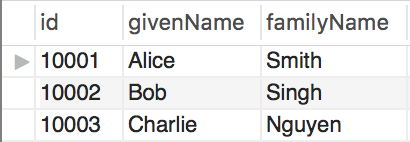
\includegraphics[width=0.5\textwidth]{q31.png}
        \caption{Results for question three}%\label{1}
        \vspace{-1em}
    \end{figure}

    {\color{red} 3 rows returned.}

    \section{ }
    \paragraph{Q4}List each student's name. For those who are in a group, list also the name of their group.
    \begin{center}
        \begin{minipage}{10cm}
        \begin{tabbing}
            \hspace*{.25in} \= \hspace*{.25in} \= \hspace*{.25in} \= \hspace*{.25in} \= \hspace*{.25in} \=\kill
            {\color{blue}SELECT `Student`.`givenName`, `Student`.`familyName`, `Groups`.`name` AS 'groupName'}\\
            \> {\color{blue}FROM `Student` LEFT OUTER JOIN `StudentInGroup`} \\
            \> {\color{blue}ON `Student`.`id` = `StudentInGroup`.`StudentId`}\\
            \> {\color{blue} LEFT OUTER JOIN `Groups` }\\
            \> {\color{blue}ON `StudentInGroup`.`groupId` = `Groups`.`id`}
        
        \end{tabbing}
        \end{minipage}
    \end{center}
    \begin{figure}[htbp!]
        \centering
        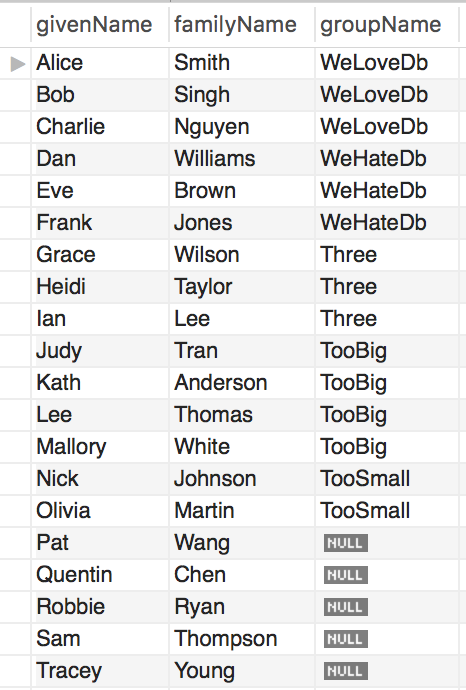
\includegraphics[width=0.5\textwidth]{q42.png}
        \caption{Results for question four}%\label{1}
        \vspace{-1em}
    \end{figure}
    {\color{red} 20 rows returned}
    \newpage
    \section{ }
    \paragraph{Q5}For any groups that have more than 3 students, list the group’s id, name and number of students.
    \begin{center}
        \begin{minipage}{10cm}
        \begin{tabbing}
            \hspace*{.25in} \= \hspace*{.25in} \= \hspace*{.25in} \= \hspace*{.25in} \= \hspace*{.25in} \=\kill
            {\color{blue}SELECT `groupId` AS 'ID of the group',`Groups`.`name` AS 'group name' , COUNT(`groupId`) AS 'number of students'}\\
            \> {\color{blue}FROM `StudentInGroup` LEFT JOIN `Groups` ON `StudentInGroup`.`groupId` = `Groups`.`id`} \\
            \> {\color{blue}GROUP BY `StudentInGroup`.`groupId`}\\
            \> {\color{blue}HAVING (COUNT(`StudentInGroup`.`groupId`) > 3) ;}\\
            %\> {\color{blue}ON `StudentInGroup`.`groupId` = `Groups`.`id`}
        
        \end{tabbing}
        \end{minipage}
    \end{center}
    \begin{figure}[htbp!]
        \centering
        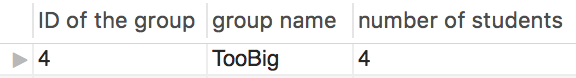
\includegraphics[width=0.5\textwidth]{q51.png}
        \caption{Results for question five}%\label{1}
        \vspace{-1em}
    \end{figure}
    {\color{red} 1 row retruned.}

    \section{ }
    \paragraph{Q6} Is student “Alice Smith” free at lunch on Wednesdays?
    \begin{center}
        \begin{minipage}{10cm}
        \begin{tabbing}
            \hspace*{.25in} \= \hspace*{.25in} \= \hspace*{.25in} \= \hspace*{.25in} \= \hspace*{.25in} \=\kill
            {\color{blue}SELECT IF(}\\
            \>{\color{blue}(SELECT * FROM }\\
            \>\> {\color{blue}(SELECT `description` 
            FROM `Student`   } \\
            \>\>\> {\color{blue}INNER JOIN `Availability` ON `Student`.`id` = `Availability`.`Student`}\\
            \>\>\> {\color{blue}INNER JOIN `Calendar` }\\
            \>\>\> {\color{blue} ON `Availability`.`day` = `Calendar`.`day` AND `Availability`.`hour` = `Calendar`.`hour` }\\
            \>\>\> {\color{blue} WHERE `givenName` = 'Alice' AND `familyName` = 'Smith') AS DT}\\
            \>\>\>{\color{blue} WHERE `DT`.`description`='lunch')  = 'lunch',}\\
            \>\> {\color{blue} 'yes', }\\
            \>\> {\color{blue} 'no'}\\
            \>{\color{blue})}\\
            \> {\color{blue} AS 'Is Alice Smith free at lunch on Wednesdays';}\\
            %\> {\color{blue}ON `StudentInGroup`.`groupId` = `Groups`.`id`}
        
        \end{tabbing}
        \end{minipage}
    \end{center}
    \begin{figure}[htbp!]
        \centering
        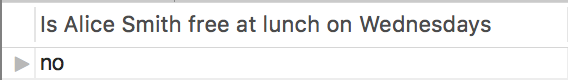
\includegraphics[width=0.5\textwidth]{q61.png}
        \caption{Results for question six}%\label{1}
        \vspace{-1em}
    \end{figure}
    {\color{red} 1 row retruned.}

    \section{ }
    \paragraph{Q7}List all times when students 10001 and 10002 are both free.
    \begin{center}
        \begin{minipage}{10cm}
        \begin{tabbing}
            \hspace*{.25in} \= \hspace*{.25in} \= \hspace*{.25in} \= \hspace*{.25in} \= \hspace*{.25in} \=\kill
            {\color{blue}SELECT `Availability`.`day`, `Availability`.`hour` FROM `Availability`}\\
            \> {\color{blue}WHERE `Availability`.`Student` = 10001} \\
            \> {\color{blue}AND (`Availability`.`day`,`Availability`.`hour`)}\\
            \> {\color{blue}IN  }\\
            \>\> {\color{blue} (SELECT `Availability`.`day`, `Availability`.`hour` FROM `Availability`}\\
            \>\> {\color{blue} WHERE `Availability`.`Student` = 10002);}\\
            %\>\> {\color{blue} 'yes', }\\
            %\>\> {\color{blue} 'no'}\\
            %\>{\color{blue})}\\
            %\> {\color{blue} AS 'Is Alice Smith free at lunch on Wednesdays';}\\
            %\> {\color{blue}ON `StudentInGroup`.`groupId` = `Groups`.`id`}
        
        \end{tabbing}
        \end{minipage}
    \end{center}
    \begin{figure}[htbp!]
        \centering
        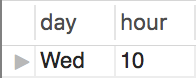
\includegraphics[width=0.4\textwidth]{q71.png}
        \caption{Results for question seven}%\label{1}
        \vspace{-1em}
    \end{figure}
    {\color{red} 1 row retruned.}

    \section{ }
    \paragraph{Q8}For each group, list the group id and name of the student whose family name is alphabetically first in the group.
    \begin{center}
        \begin{minipage}{10cm}
        \begin{tabbing}
            \hspace*{.25in} \= \hspace*{.25in} \= \hspace*{.25in} \= \hspace*{.25in} \= \hspace*{.25in} \=\kill
            {\color{blue}SELECT `groupId`, `givenName`, `familyName` FROM}\\
            \>\>{\color{blue}(SELECT
            `groupId`, `givenName`, `familyName` 
            FROM `StudentInGroup`}\\
            \>\>\>{\color{blue} LEFT JOIN `Student` ON `StudentInGroup`.`StudentId`=`Student`.`id`}\\
            \>\>\>{\color{blue} ORDER BY `groupId`, `familyName` DESC)
            AS t1 }\\
            \>{\color{blue} LEFT JOIN}\\
            \>\>{\color{blue} (SELECT `groupId` AS gID, `givenName` AS ggN, `familyName` AS fN}\\
            \>\>\>{\color{blue} FROM `StudentInGroup` LEFT JOIN `Student` ON `StudentInGroup`.`StudentId`=`Student`.`id`}\\
            \>\>\>{\color{blue} ORDER BY `groupId`, `familyName` DESC)
            AS t2}\\
            \>{\color{blue} ON t1.`groupId` = t2.`gID` AND t1.`familyName` > t2.`fN`}\\
            \>{\color{blue} WHERE t2.`gID` IS NULL}\\
            \>{\color{blue} ORDER BY 1;}
        \end{tabbing}
        \end{minipage}
    \end{center}
    \begin{figure}[htbp!]
        \centering
        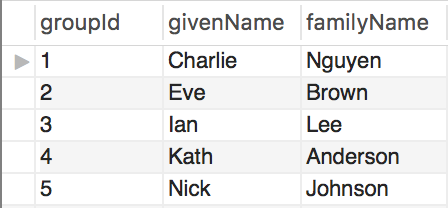
\includegraphics[width=0.4\textwidth]{q81.png}
        \caption{Results for question eight}%\label{1}
        \vspace{-1em}
    \end{figure}
    {\color{red} 5 rows retruned.}

    \section{ }
    \paragraph{Q9} Which students are free on Wednesdays between 10am and 12 noon? Show their ids and names.
    \begin{center}
        \begin{minipage}{10cm}
        \begin{tabbing}
            \hspace*{.25in} \= \hspace*{.25in} \= \hspace*{.25in} \= \hspace*{.25in} \= \hspace*{.25in} \=\kill
            {\color{blue}SELECT `id`, `givenName`, `familyName` FROM}\\
            \>{\color{blue}(SELECT *}\\
            \>\>{\color{blue}FROM `Student` AS S INNER JOIN `Availability` AS AVA ON  `S`.`id`=`AVA`.`Student`}\\
           \>\> {\color{blue}WHERE `AVA`.`day` = 'Wed' }\\
            \>\>{\color{blue}AND `AVA`.`hour` BETWEEN 10 AND 11 ) AS DT}\\
            \>{\color{blue}WHERE `DT`.`hour` = 11;}

        
        \end{tabbing}
        \end{minipage}
    \end{center}
    \begin{figure}[htbp!]
        \centering
        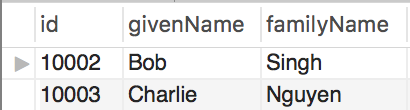
\includegraphics[width=0.4\textwidth]{q91.png}
        \caption{Results for question nine}%\label{1}
        \vspace{-1em}
    \end{figure}
    {\color{red} 2 rows retruned.}

    \section{ }
    \paragraph{Q10} Are the members of 'WeLoveDb' all free on Wednesday at 10am?
    \begin{center}
        \begin{minipage}{10cm}
        \begin{tabbing}
            \hspace*{.25in} \= \hspace*{.25in} \= \hspace*{.25in} \= \hspace*{.25in} \= \hspace*{.25in} \=\kill
            {\color{blue}SELECT IF(}\\
            \>\>{\color{blue}(SELECT COUNT(*) FROM `StudentInGroup`}\\
            \>\>\>{\color{blue} INNER JOIN `Groups`}\\
            \>\>\>{\color{blue} ON `StudentInGroup`.`groupId` = `Groups`.`id` WHERE `Groups`.`name`='WeLoveDb')}\\
            \>\>{\color{blue} =}\\
            \>\>{\color{blue} (SELECT COUNT(*) FROM `StudentInGroup`}\\  
            \>\>\>{\color{blue} INNER JOIN `Groups` ON `StudentInGroup`.`groupId` = `Groups`.`id` }\\
            \>\>\>{\color{blue} INNER JOIN `Availability` ON `Availability`.`Student`=`StudentInGroup`.`StudentId`}\\
            \>\>\>{\color{blue} WHERE `Groups`.`name`='WeLoveDb' AND `Availability`.`day`='Wed' AND `Availability`.`hour`=10),}\\
            \>\>{\color{blue}'yes',}\\
            \>\>{\color{blue}'no'}\\
            \>\>{\color{blue})}\\
            \>{\color{blue}AS 'Are the members of $\backslash$'WeLoveDb $\backslash$' all free on Wednesday at 10am?';}
        \end{tabbing}
        \end{minipage}
    \end{center}

    \begin{figure}[htbp!]
        \centering
        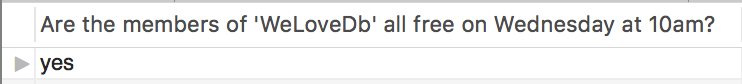
\includegraphics[width=0.4\textwidth]{q101.png}
        \caption{Results for question ten}%\label{1}
        \vspace{-1em}
    \end{figure}
    {\color{red} 1 row retruned.}



    \end{document}
    
    
    
    %\begin{align} 
    %\begin{split}
    %(x+y)^3 	&= (x+y)^2(x+y)\\
    %&=(x^2+2xy+y^2)(x+y)\\
    %&=(x^3+2x^2y+xy^2) + (x^2y+2xy^2+y^3)\\
    %&=x^3+3x^2y+3xy^2+y^3
    %\end{split}					
    %\end{align}
    
    
    
    
    
    %\begin{tabbing}
    %\hspace*{.25in} \= \hspace*{.25in} \= \hspace*{.25in} \= \hspace*{.25in} \= \hspace*{.25in} \=\kill
    %\>$Euclid(m,n)=$ \\
    %\>\> {\bf while} n$ \neq $ 0 \\
    %\>\>\> r $ \leftarrow $ $m$ mod $n$  \\
    %\>\>\>  m $\leftarrow$n\\
    %\>\>{\bf return} m 
    %\end{tabbing}
    
    %Python code:
    %\begin{lstlisting}[language = python]
    %def gcd(m,n):
    %	while n != 0:
    %		r = m % n
    %		m = n
    %		n = r
    %	return m
    %\end{lstlisting}
    
    
    %\paragraph{Heading on level 4 (paragraph)}
    
    
    
    
    %\begin{tabbing}
    %	\hspace*{.25in} \= \hspace*{.25in} \= \hspace*{.25in} \= \hspace*{.25in} \= \hspace*{.25in} \=\kill
    %	{\bf function} find (A,x,n)\\
    %	\> j $\leftarrow$ 0\\
    %	\> {\bf while} j < n\\
    %	\>\> {\bf if} A[j]=x\\
    %	\>\>\>  {\bf return} j  \\
    %	\>\> j $\leftarrow$ j+1\\
    %	\> {\bf return} -1
    %\end{tabbing}
    
    
    %\begin{figure}[htbp!]
    %		\centering
    %		\includegraphics[width=0.6\textwidth]{lec26.png}
    %		\caption{Linked List}%\label{book}
    %		\vspace{-1em}
    %\end{figure}
    
    
    
    
    
    
    %\begin{align}
    %A = 
    %\begin{bmatrix}
    %A_{11} & A_{21} \\
    %A_{21} & A_{22}
    %\end{bmatrix}
    %\end{align}
    
    
    
    %\begin{algorithm}
     %       \caption{Count the number of occurrences of a certain integer $x$ in an array $A[]$}
      %      \begin{algorithmic}[1] %每行显示行号
       %         \Require  $Array$ A[],$Length\;of\;the\;array$ n, $Integer$ x
        %        \Ensure   Number of occurrence of integer x  
         %       \Function {NumberCount}{$A[], x,n$}
          %      
           %     	\State $firstApperence \gets $\Call{FirstOccurrenceSearch}{$A[]$,0,$n-1$,$x$,$n$}
                    
            %    	\If{$firstApperence=-1$}
             %   	\State \Return $firstApperence$
              %  	\EndIf
                    
               % 	\State $lastApperence\gets$ \Call{LastOccurrenceSearch}{$A[],firstApperence,n-1,x,n$}
                %	\State \Return $lastApperence-firstApperence+1$
                    
                    %\State $result \gets 0$
                    
                    %\If {$high \geqslant low$}
                        %\State $mid \gets (high + low) // 2$   \#"//" means integer division
                        %\State $result \gets result +$ \Call{MergerSort}{$Array, left, middle$}
                        %\State $result \gets result +$ \Call{MergerSort}{$Array, middle, right$}
                        %\State $result \gets result +$ \Call{Merger}{$Array,left,middle,right$}
                    %\EndIf
                    %\If {$mid = 0 \, OR x > A[mid-1]$}
                    %	\State \Return $mid$
                    %\Else 
                    %	\If {$x>A[mid]$}
                    %		\State \Return 
                    
                     %\Return{$result$}
                %\EndFunction
               %\State
                %\Function{FirstOccurrenceSearch}{$A[],low, high,x,n$}
                
          %      \If{$high \geqslant low$}
          %      \State $mid\gets(low + high)//2$ \Comment "//" means integer division
          %      \EndIf
          %      \If{$\{mid = 0 \; OR\;  x>A[mid-1]\}\; AND\; \{A[mid]=x\}$} 
          %      \State \Return $mid$
          %      \Else
          %      	\If{$x>A[mid]$}
          %      	\State \Return \Call{FirstOccurrenceSearch}{$A[],mid+1,high,x,n$}
          %      	\Else
          %      	\State \Return \Call{FirstOccurrenceSearch}{$A[],low,mid-1,x,n$}
          %      	\EndIf
          %      \EndIf
          %      \State \Return -1
          %      
          %      \EndFunction
          %      
          %      \State
          %      \Function{LastOccurrenceSearch}{$A[],low,high,x,n$}
          %      
          %      \If{$high \geqslant low$}
          %      \State $mid\gets(low + high)//2$ \Comment "//" means integer division
          %      \EndIf
          %      \If{$\{mid = n-1 \; OR\;  x<A[mid-1]\}\; AND\; \{A[mid]=x\}$} 
          %      \State \Return $mid$
          %     \Else
           %     	\If{$x<A[mid]$}
            %    	\State \Return \Call{LastOccurrenceSearch}{$A[],low, mid-1, x,n$}
             %   	\Else
              %  	\State \Return \Call{LastOccurrenceSearch}{$A[],mid+1, high,x,n$}
               % 	\EndIf
                %\EndIf
                %\State \Return -1
                
                
    
               % \EndFunction
                
                %\Function{Merger}{$Array, left, middle, right$}
                 %   \State $i\gets left$
                  %  \State $j\gets middle$
                   % \State $k\gets 0$
                   % \State $result \gets 0$
                   % \While{$i<middle$ \textbf{and} $j<right$}
                    %    \If{$Array[i]<Array[j]$}
                     %       \State $B[k++]\gets Array[i++]$
                      %  \Else
                       %     \State $B[k++] \gets Array[j++]$
                        %    \State $result \gets result + (middle - i)$
                        %\EndIf
                    %\EndWhile
                    %\While{$i<middle$}
                    %    \State $B[k++] \gets Array[i++]$
                    %\EndWhile
                    %\While{$j<right$}
                    %    \State $B[k++] \gets Array[j++]$
                    %\EndWhile
                    %\For{$i = 0 \to k-1$}
                    %    \State $Array[left + i] \gets B[i]$
                    %\EndFor
                    %\State \Return{$result$}
                %\EndFunction
          %  \end{algorithmic}
        %\end{algorithm}
    
    
    
    
    
    